\documentclass[a4paper,12pt]{article}
\usepackage{graphicx}
\usepackage[hungarian]{babel}
\usepackage[T1]{fontenc}
\usepackage[utf8]{inputenc}
\usepackage{multirow}
\usepackage{amsmath}
\usepackage{float}
\usepackage{enumerate}
\usepackage{caption}
\usepackage{subcaption}
\usepackage{indentfirst}
\usepackage{color}
\usepackage{array}
\bibliographystyle{unsrt}
\usepackage[top=4cm ,bottom=4cm ,left=3cm ,right=3cm]{geometry}
\usepackage{multirow}
\usepackage{url}
\usepackage{listings}
\usepackage{color}

\definecolor{codegreen}{rgb}{0,0.6,0}
\definecolor{codegray}{rgb}{0.5,0.5,0.5}
\definecolor{codepurple}{rgb}{0.58,0,0.82}
\definecolor{backcolour}{rgb}{0.95,0.95,0.92}

\lstdefinestyle{mystyle}{
	backgroundcolor=\color{backcolour},   
	commentstyle=\color{codegreen},
	keywordstyle=\color{magenta},
	numberstyle=\tiny\color{codegray},
	stringstyle=\color{codepurple},
	basicstyle=\footnotesize,
	breakatwhitespace=false,         
	breaklines=true,                 
	captionpos=b,                    
	keepspaces=true,                 
	numbers=left,                    
	numbersep=2pt,                  
	showspaces=false,                
	showstringspaces=false,
	showtabs=false,                  
	tabsize=2
}

\lstset{style=mystyle}

\author{Alex Olar}
\title{CBM szimuláció}
\date{\today}

\begin{document}
\maketitle
\vfill
\begin{center}
	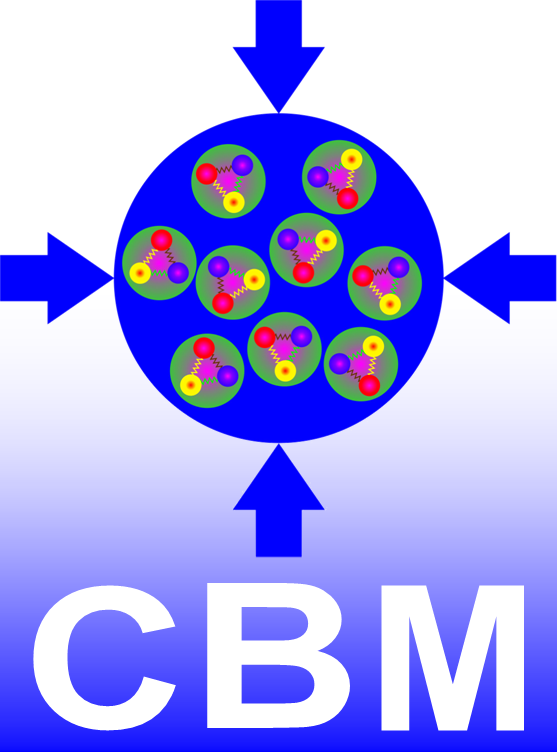
\includegraphics[width=0.66\textwidth]{gsi.png}
\end{center}
\newpage
\renewcommand{\abstractname}{Bevezető}
\renewcommand{\thesection}{\Roman{section}.}
\renewcommand{\thesubsection}{\thesection\arabic{subsection}}
\renewcommand{\thesubsubsection}{\thesubsection\arabic{subsubsection}}
\begin{abstract}
	\par Egy hónapot töltöttem a nyár folyamán, július hónapba, Darmstadtban a GSI nevű kutatóközpontban. Kint tartózkodásom célja az volt, hogy többet megtudjam a  CBM saját szimulációjáról, amely kutató csoport már az épülő FAIR\footnote{ Facility for Antiproton and Ion Research } része. Ezalatt a hónap alatt megismerkedtem mélyebben a ROOT \footnote{ CERN szoftver részecske analízishez} nevű szoftverrel, a helyi cbmROOT-tal \footnote{ CBM ( Compressed Barionic Matter  ) szoftver a GSI/FAIR által fejlesztve}, valamint a C és C++ programozási nyelvekkel.
	\vspace{5mm}
	\par A kint létem alatt sokat tanultam a detektor technológiákról, valamint az azokban lejátszódó eseményekről és örömmel voltam részese ennek a nagyszabású projektnek és a mindennapi kutatói életnek.
\end{abstract}
\tableofcontents
\newpage
\section{ Alapok}
\subsection{ QCD - BSc-s szemmel}
\vspace{5mm}
\par A 20. század folyamán fizikusok szembeszültek azzal, hogy milyen abszolút fontos szerepet töltenek be a szimmetriák az univerzum és a körülöttünk lévő világ megismerésében. A szimmetriák vezették el őket a megmaradási tételekig, valamint az antirészecskék és kvarkok felfedezéséig többek között. 
\vspace{5mm}
\par A kvarkok felfedezése végre rendett teremtett a részecske állatkertben (particle ZOO), ahogy az elemi részecskék folyamatosan növő számára Niels Nohr szellemsen referált.  Kezdetben csak három kvark volt ismert, úgy mint: $\textsl{u}$ (up), $\textsl{d}$ (down), $\textsl{s}$ (strange). A hadronok két csoportba oszthatók szét: $\textsl{mezonok}$ és $\textsl{barionok}$, amelyek rendre egy kvark-antikvark párt vagy három kvarkot tartalmaznak. A mennyiséget ami a különböző kvarkokat bizonyos szempontból jellemzi $\textsl{íz}$nek hívjuk.
\vspace{5mm}
\par Az erős kölcsönhatás, ami a kvarkok között ható elemi kölcsönhatás, egyedi tulajdonsága a bezárás, ami megakadályozza a kvarkokat abban, hogy elszeparálva, izoláltan megtalálhatóak legyenek. Az erős kölcsönhatás töltését színnek hívjuk. A bezárás miatt, az elemi részecskék csak úgynevezett semleges színben létezhet, amit gyakran `fehérnek' nevezünk. Az erőskölcsönhatást leíró alapvető elmélet a Kvantumszíndinamika (Quantum Chromo Dynamics) - QCD.
\vspace{5mm}
\par A QCD elemi részecskéi a kvarkok és antikvarkok, amelyek a gluonok által hatnak kölcsön, melyek szinén színtöltést holdoznak. A gluonoknak 8 fajtájuk van, hogy minden színtranszfromáció leírható legyen segítségükkel. A gluonok önmagukkal is kölcsön tudnak hatni.
\subsection{ CBM fizika }
\vspace{5mm}
\par A barionanyaggal foglalkozva az elsődleges cél, hogy megértsük és jobban megismerjük a fázisátmenetekhez tartozó diagramot és magukat az átmeneti folyamatokat.
Először is rövid bevezetőként egy kis termodinamikai áttekintéssel kezdek a fázisokról és a fazisátalakulásokról, alapul véve a The CBM Book-ot:
\vspace{5mm}
\par A víz fázisdiagramja megmutatja annak külöböző fáziasait egy nyomás-hőmérséklet rendszerben. Ismeretes, hogy adott körülmények között van egy
hármaspont, amelyben a víz mindhárom halmazállapotában előfordul. A fázisok közötti vonalak mentén a víz szintén több (itt kettő) halmazállapotban
előfordulhat és ezek kölcsönösen megtalálhatóak a megfelelő körülmények között. Elsőrendű fázisátmenetnek hívjuk, amikor ezen vonalakon `áthaladva' halmazállapot-változás
történik. Továbbá megkülönböztetünk egy kritikus pontot is, amely után a fázisok nem különülnek el jelentős mértékben, ezután
csak egy úgynevezett sima $\textsl{crossover}$ figyelhető meg, nem elsőrendű fázisátmenet.
\begin{figure}[H]
	\centering
	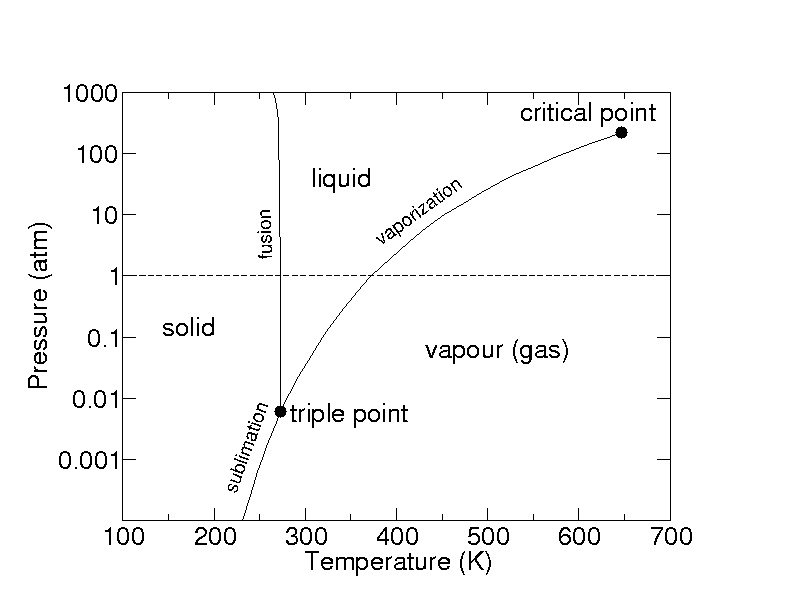
\includegraphics[width=0.76\textwidth]{water_phase.jpg}
	\caption{ A víz fázisdiagramja. }
\end{figure}
\par Most, hogy gyorsan áttekintettem a víz fázisdiagramját, vagy legalábbis egy részét, ideje továbblépni és feltenni a kérdést, hogy mi 
a helyzet az erősen kölcsönható anyaggal. Az erősen kölcsönható anyag fázisdiagramja ugyanis elméleti stádiumban van, még nincs teljesen
kísérletileg bizonyítva. Az ábrákon olyan különböző és elengedhetetlenül fontos fázisok vannak, amelyek a korai univerzumot jellemezték vagy éppen
a neutron csillagok anyagát alkothatják. Itt mindkét ábrán egy hőmérséklet-sűrűség diagramot láthatunk.
\begin{figure}[H]
	\centering
	\begin{subfigure}{.49\textwidth}
		\centering
		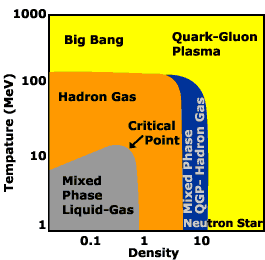
\includegraphics[width=0.92\textwidth]{cbm_phase1.png}
		\caption{ Hőmérséklet MeV-ban kifejezve, míg a sűrűség magsűrűségben van megadva, mindkét skála logaritmikus }
	\end{subfigure}
	\begin{subfigure}{.49\textwidth}
		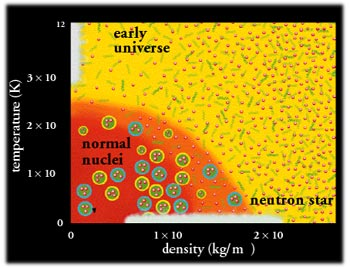
\includegraphics[width=.92\textwidth]{cbm_phase2.jpg}
		\caption{ Ezen a diagramon a fázisok természetbeli előfordulását láthatjuk. }
	\end{subfigure}
\end{figure}
\par A fentebbi ábrákon is látható egy fázis, amit kvark-gluon plazmának nevezünk. Ez az állapot jelen volt a Nagy Bummnál, de később
nem maradt fenn, a hőmérséklet hirtelen csökkenése miatt. Látható az is, hogy a neutron csillagok belseje is kvark-gluon plazmát tartalmazhat,
de azokban nem a hőmérséklet kell igen magas legyen, hanem a csillag sűrűsége. 
\vspace{5mm}
\par Nyilvánvalóan, a kvark-gluon plazma földi megfigyelésének egyetlen lehetőségét a nagy energiás részecske gyorsítók és azok
ütköztetése biztosítja. A QCD jellemző tulajdonsága, hogy a kvarkok közti összetartás csökken, ahogy az ütközési energiát
növeljük, ez a crossover jelensége. A szakirodalom aszimptotikus szabadságként hivatkozik rá. A részecske fizika egy másik fontos
szimmetriája a kiralitással kapcsolatos. Ez lényegében arról beszél, hogy egy tömegtelen részecske spinje és sebességének iránya egymáshoz 
képest milyen irányba mutat. Hogyha azok egyirányúak, akkor a részecske jobb kezes, ha ellentétes irányúak akkor pedig bal kezes. Mivel
az up és down kvarkok tömege közel azonos, ezért azt szokták mondani, hogy a QCD-nek körülbelüli királis szimmetriája van. Ellenben, ez spontán
sérülhet alacsony hőmérsékleteken és sűrűségeken, ahol ez a kicsi tömegbeli különbség is jelentős lehet. Emiatt az egyik királis irány ekkor 
gyakoribb lesz, mint a másik, ezt nevezzük lényegében királis szimmetriasértésnek. 
\section{ A CBM detektor}
\subsection{ Elmélet}
\vspace{5mm}
\par A nehézionok ütközésének vizsgálata és az adatok feldolgozása egy borzasztóan komplex feladat a reakció tranziens természete miatt. 
Lényegében az a cél, hogy az ütközés során, $10^{-22}~s$-ig fennálló állapot segítségébel következtessünk az erősen kölcsönható anyag 
fázisdiagramjára, a jelenség természetére. Az idő természetesen nagyon rövid, és az egész jelenség csak a melléktermékek révén vizsgálható. 
\par  Az elmúlt évtizedben a fő tudományos tevékenység a témában a brookheaven-i RHIC  \footnote{ Relativistic Heavy Ion Collider - Brookhaven } központban 
és a CERN-ben található LHC \footnote{ CERN - Large Hadron Collider } gyorsítónál zajlott. Ezek a központok nagyon fontos, és érdemleges 
adatot biztosítanak a fázisdiagram vizsgálatához. Ellenben ezek mind az alacsony sűrűségű régiót vizsgálják és csak a crossovert tudják
feltérképezni a hadron gáz és a kvark-gluon plazma között. A FAIR projekt ezekkel szemben sokkal magasabb barion sűrűséget tervez elérni, hogy 
lehetőséget biztosíton az első rendű fázisátmenet vizsgálatára, valamint a kritikus pont környékének feltérképezésére. 
\begin{figure}[H]
	\centering
	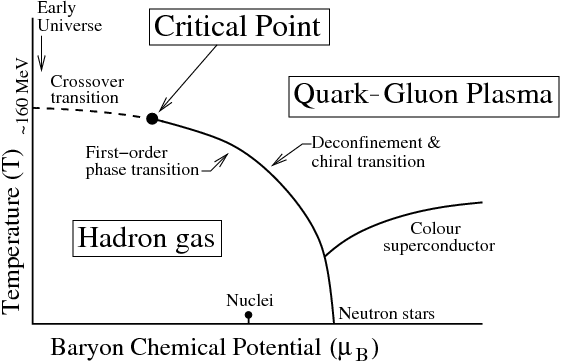
\includegraphics[width=0.96\textwidth]{CBM_phase_trans.png}
	\caption{ A fentebb említett elméleti fázisdiagram  }
\end{figure}
\subsection{ Detektor elrendezés és a szimuláció}
\par A detektor elrendezése balról jobbra haladva a következő (ábra):
\begin{itemize}
	\item CBM szupravezető mágnes szilícium sprektrométerrel
	\item a micro vertex detektor ( MVD ) az előbbi belsejében
	\item a szilícium követő rendszer ( STS ) is
	\item Cserenkov-detektor ( RICH - ring imaging Cherenkov detector - világos kék )
	\item ezt követi 4 réteg átmeneti sugázás ( TRD - transition radiation detector ) detektor
	\item és egy time-of-flight ( TOF ) fal
	\item a fő detektorok után található még egy müon sprektrométer és egy célfigyelő detektor (PSD)  
\end{itemize}
\begin{figure}[H]
	\centering
	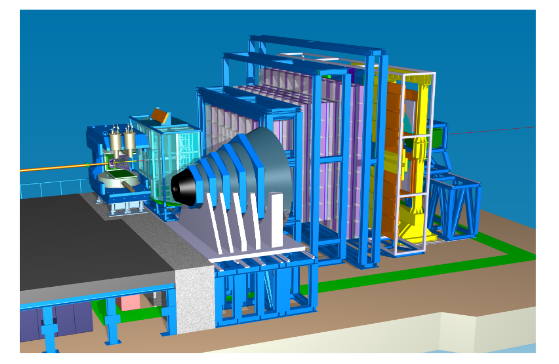
\includegraphics[width=0.66\textwidth]{cbm_detector.png}
	\caption{ A detektor elrendezés }
\end{figure}
\par A szilícium követő rendszer feladata az, hogy rekonstruálja majd a részecskék trajektóriáit. Csak töltött részecskék észlelésére képes, 
de képes mérni a töltés nagyságát és az impulzust is tud mérni. A TOF fal igen nagy felbontást tud elérni, nagyjából 60 ps-os felbontásra is
lehetőség van.
\vspace{5mm}
\par A CBM projekt még egyenlőre csak terv szintjén létezik, a szimulációt folyamatosan fejlesztik. Jövőre, vagy legkésőbb 2019-re már tervben 
van egy miniCBM detektor építése az esetleg később felmerülő tervezési, kivitelezési proglémák kivitelezésére. A FAIR létesítmény építése idén 
nyáron kezdődött és az első részecskenyaláb 2022-ben várható. A miniCBM projekt a meglévő GSI gyorsítónál fog tevékenykedni az addig fennmaradó
időben, ahol megpróbálják a számítógépfarmot tökéletesíteni, hogy az adatokat minél gyorsabban feldolgozhassák.
\vspace{5mm}
\par A FAIR tudósai kifejlesztettek egy több tízezer soros szimulációt, ami a ROOT-on alapszik. Ezt ők cbmROOT-nak hívják, mivel teljes
egészében a CBM-hez igazodik és ingyenesen elérhető bárki számára. Sok jól ismert nehézion szimulációs eljárást használnak, amik a CBM
környeztre vannak szabva, úgy mint: UrQMD \footnote{ Ultra Relativistic Quantum Molecular Dynamics }, valamint  PHSD \footnote{ Parton Hadron String Dynamics }.
 Ezek a szimulációs kódok széles körben használtak nem csak itt, hanem az egész tudomány területen. 
\section{ A $\Phi$-mezonról röviden}
\subsection{ $\Phi$-mezon rekonstrukció}
\vspace{5mm}
\par A CBM detekter egy általános célú nehézion mérési eszköz lesz, hogy az erősen kölcsönható anyag fázisdiagramját vizsgálni lehessen. A
rezonanciák nagyon fontosak, hogy a sűrű anyagot vizsgálni tudjuk az ütközés során. Az ilyen rezonanciák egyike ami fontos a CBM és a 
fázisdiagram vizsgálatának szempontjából pedig a $\Phi$-mezon, aminek nagyon kicsi a hadronokra vett hatáskeresztmetszete így eléggé 
valószínűtlen, hogy kölcsönhat a nagy mennyiségű hadronnal, ami a reakció során keletkezik, vagyis jó indikátora a sűrű, kezdeti eseménynek.
A $\Phi$-mezon egy strange és egy anti-strange kvarkot tartalmaz és a kulcsa lehet az s kvark partonikus anyagban lévő keletkezésére. A
$\Phi$-mezon $K^{+}, K^{-}$ párokra bomlik nagyjából 50$\%$-os eséllyel és egyebekre (pl. dileptonokra is). Az közepes élettartama egészen
kicsi, nagyjából $1.55\cdot10^{-22}$ s tehát még a TOF falat sem éri el, csak a bomlástermékei lesznek detektálva már korábban is. 
A tömege $1.019$ MeV ami a kaonok invariáns tömegével kifejezve egy rezonancia csúcsként látható az ütközés/szimuláció után kinyert 
adatok között. 
\vspace{5mm}
\par Én a PHSD adatait vizsgáltam, amin lefuttattam a CBM szimulációt. Egy Au+Au centrális ütközést vizsgáltam $\sqrt{s} = 10$ GeV energián. 
A CBM szimuláció kimenetét a cbmROOT-tal rekonstruáltam. Több mint 5 millió esemény szerepelt a kezdeti $.root$ fájlban amit a szimulációhoz 
használtam.
\vspace{5mm}
\par A hisztogramokon az x-tengelyen a kaon párok invariáns tömege szerepel, az y-tengelyen pedig az adott energián a `beütések' száma. Egy 
apró kiugrás látható a nagy kombinatorikus háttéren nagyjából $1.02$ GeV környékén ami pontosan a $\Phi$-mezonra utal. Azok voltak
a keletkezett $\Phi$-mezonok az ütközés során. 
\begin{figure}[H]
	\centering
	\begin{subfigure}{0.49\textwidth}
		\centering
		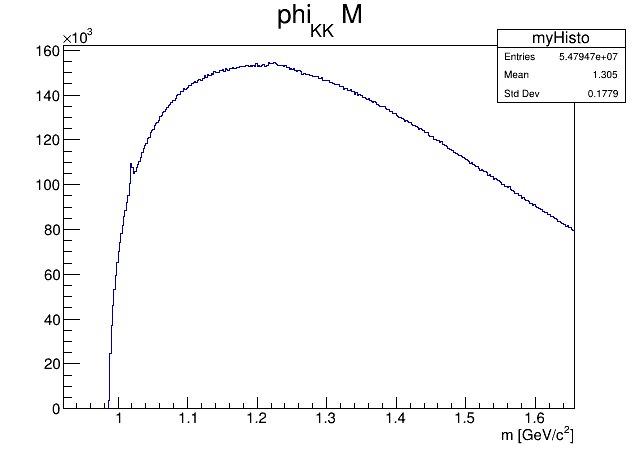
\includegraphics[width=0.95\textwidth]{phi_KK_M.png}
		\caption{ A kombinatorikus háttér és egy apró, de jól látható csúcs. }
	\end{subfigure}
	\begin{subfigure}{0.49\textwidth}
		\centering
		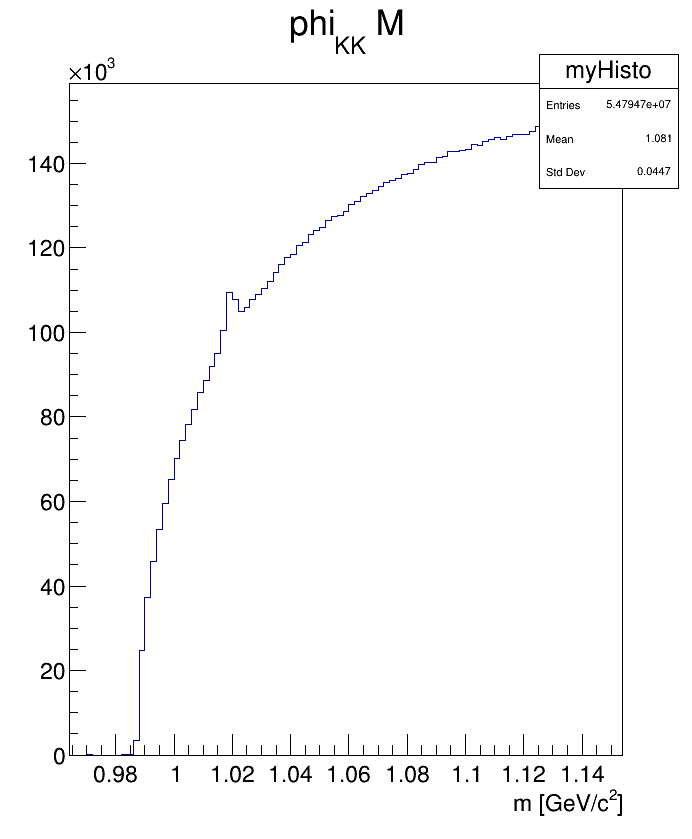
\includegraphics[width=0.95\textwidth]{phi_KK_Mzoom.png}
		\caption{ A csúcs. }
	\end{subfigure}
\end{figure}
\par Egy másodfokú polinommal próbáltam becsülni a hátteret. Az illesztés paraméterei ($ax^{2} + bx +c$) :
\begin{center}
	\begin{tabular}{|c|c|c|}
		\hline
		Parameter name & Value []     & Error   \\
		\hline
		a              & -7.70559e+06 & 78750.5 \\
		\hline
		b              & 1.42738e+07  & 150055  \\
		\hline
		c              & -6.49147e+06 & 71438.9 \\
		\hline
	\end{tabular}
\end{center}
\par A háttér illesztése: 
\begin{figure}[H]
	\centering
	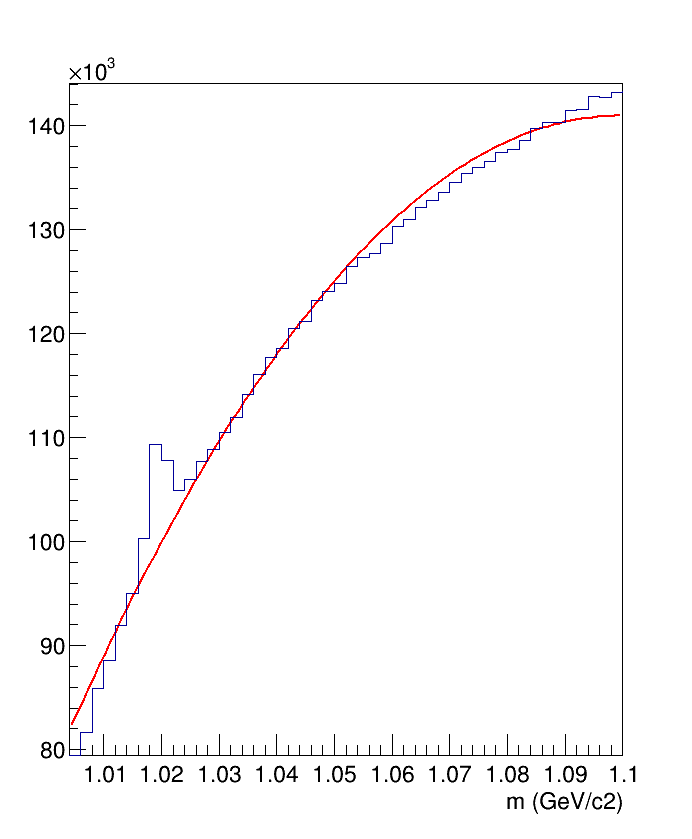
\includegraphics[width=0.35\textwidth]{combiback_fit.png}
	\caption{ A háttérre vett illsztés a másodfokú polinommal. }
\end{figure}
\par A csúcshoz más módszert alkalmaztam. Egy alacsony multiplicitású jelet használtam a csúcs alakjának becsléséhez, amit egy
Gauss-függvénnyel illesztettem, majd ezt skáláztam fel a csúcshoz, az állandó nagyságú háttér mellett, az eredmények a következők:
\begin{figure}[H]
	\centering
	\begin{subfigure}{0.49\textwidth}
		\centering
		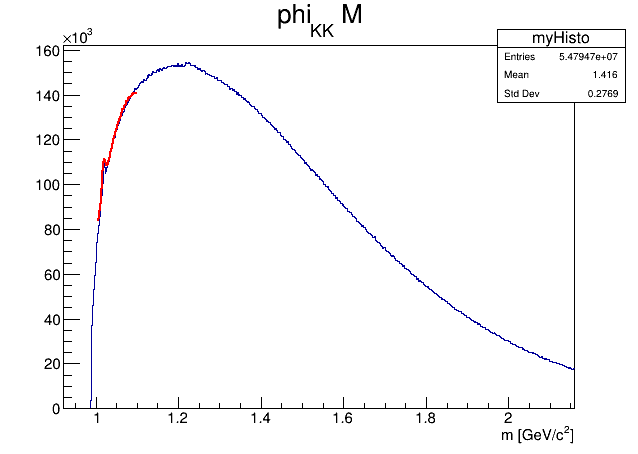
\includegraphics[width=0.95\textwidth]{phi_KK_Mfit.png}
		\caption{ A háttér és a csúcs illesztése. }
	\end{subfigure}
	\begin{subfigure}{0.49\textwidth}
		\centering
		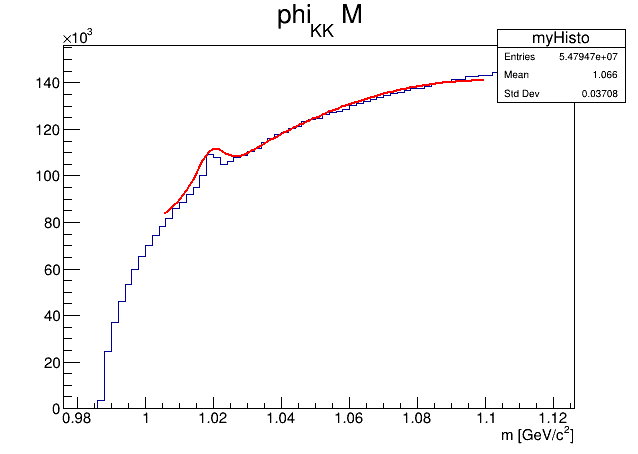
\includegraphics[width=0.95\textwidth]{phi_KK_Mfitzoom.png}
		\caption{ Ráközelítve. }
	\end{subfigure}
\end{figure}
\par Itt a ROOT makróm, amit az `illesztéshez' használtam:
\lstinputlisting[language=C++]{fit.C}
\subsection{$\Phi$-mezon a CBM-ben}
\vspace{5mm}
\par Igen nehéz feladat lesz hatékonyan detektálni a $\Phi$-mezonokat a CBM detektorrendszerrel. A részecskék nem csak rövid 
életűek, de egy hatalmas háttér is nehezíti az apró csúcs megtalálását. Ezért is kell hatalmas számú eseményt vizsgálni, hogy a csúcs
a statisztikában már látható legyen. Ennek ellénre határozottan mondhatjuk, hogy a CBM detektor képes lesz a $\Phi$-mezonok detektálására
és ezáltal a strange kvark termelődésénék megértésére az erősen kölcsönható anyagban.
\vspace{5mm}
\par A szimuláció hatékonysági mutatókat is biztosít. Mindezeket különböző részecske impulzusok esetén. A jelzett detektálás 
hatékonysági értékek nem túl magasak, de eléggé stabilak adott tartományokban az észleléshez:
\begin{figure}[H]
	\centering
	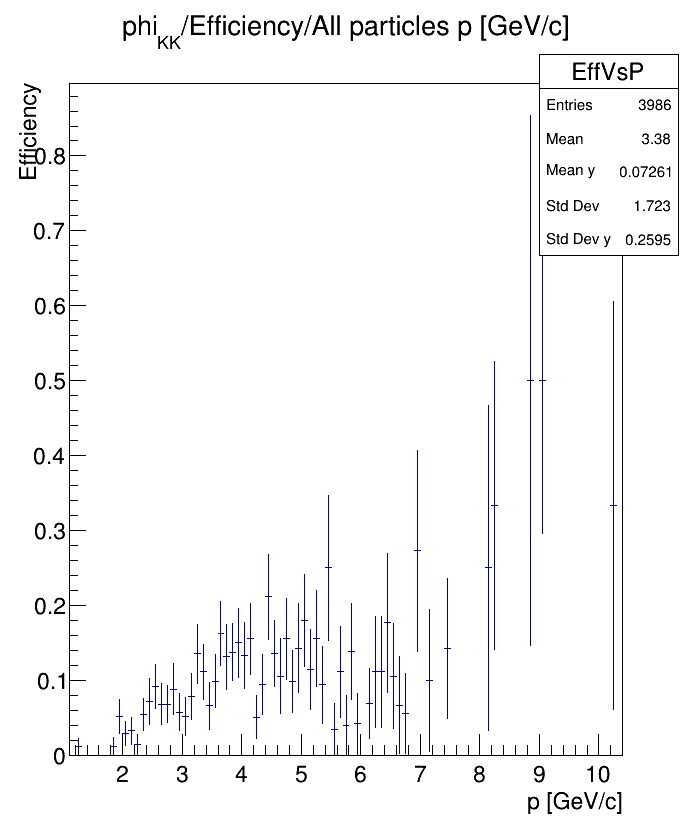
\includegraphics[width=0.65\textwidth]{efficieny.png}
	\caption{ Hatékonyság az impulzus függvényében }
\end{figure}
\section{ A szimuláció}
\vspace{3mm}
\subsection{ Telepítés}
\vspace{5mm}
\par A CBM szimuláció telepítésénék három fő komponense van, az egyik a FairROOT, majd a FairSoft és végül a cbmROOT. Bármilyen 
rendszerre telepíthetőek az alábbi linkről:
\url{https://redmine.cbm.gsi.de/projects/cbmroot/wiki/InstallCbmRootAuto} \newline
\par Erősen ajánlott a telepítést ezt követve megtenni, mivel rengeteg apró, de akadályozó probléma előjöhet a telepítés során. A teljes
csomag tartalmazza a ROOT-ot is, így az egész nagyjából 25 GB helyet foglal. 
\subsection{ Bevezetés}
\vspace{5mm}
\par Maga az ütközés a UrQMD és a PHSD programok segítségével játszódik le, a CBM szimuláció a detektor választ szimulálja, tehát az ezekből
származó adatokat kapja meg kezdeti paraméternek. Ezek a modellek az ALICE, RHIC és LHC detektornak, valamint nem utolsó sorban a
CBM detektornak lettek fejlesztve. Én főleg UrQMD adatokat használtam, de PHSD fájlokkal is találkoztam kintlétem során. 
\vspace{5mm}
\par Az első lépés az, hogy le kell futtatni egy Monte Carlo szimulációt, hogy képeset legyünk a `valódi' adatokat összepárosítani a 
keltett eseményekkel. A program ezen része arra lett tervezve, hogy kiszűrje a találatokat a detektor anyagban és olyan pontokat találjon, 
amelyek később trajektóriákká összeállíthatók.
\vspace{5mm}
\par A program a Geant3 és Geant4 programokat használja, hogy a részecskék anyagon való áthaladását szimulálja. Ez is a Monte Carlo 
szimuláció része.
\vspace{5mm}
\par Az első makró kimenetén tehát egy szimulációs fájl van, ami az STS és az MVD detektorok által detektált találaltokat tartalmazza 
valamint a TOF fal és egyéb detektok adatait is. Ezeket felhasználva lép a program a második fázisba, a rekonstrució részhez. A rekonstrukciós 
kód először is klasztereket próbál találni az MVD detektorban, hogy megtalálja, hogy hol volt az ütközés/ütközések kiinduló pontja. Ha ezt megtalálta
továbbhalad és megpróbálja lekövetni a részecske pályákat. A tölött részecskék körpályára állnak az erős mágneses tér hatására így a pontokra
köríveket próbálnak illeszteni és a legjobb illesztéssel bírókat fogadják csak el (van egy százalékos határ, ami alatt hibás detektálásnak ítélik). Én főleg
az MVD és STD detektorokra koncentráltam, tehát a többit most nem említem itt.
\vspace{5mm}
\par Nyilvánvalóan, a találaltok és a pályákat többször próbálja meg a program helyesen megtalálni, azért, hogy elkerülje a hibákat. Kisebb
az esélye így a hibás találatnak, vagy a hibásan illesztett trajektóriának. Ennék része a digitalizáció, ami lényegében azt jelenti, hogy a 
szimulációs program megpróbálja a detektor választ is számításba venni. Vegyük például az STS detektort. Ennek egy szálas, hálós elrendezése 
van, amikor egy részecske áthalad, akkor több szálban is detektálju, ezek metszéspontjában van a tényleges helye. De ha egyszerre két
részecske ment át `ugyan azon a ponton', akkor ezt nem láthatjuk, később a pályák illesztésénel probléma lehet. Ezért is van az, hogy ha
az STS detektor több, mint 5$\%$-a detektál, akkor a rendszer lényegében nem mér, nem szerez kiértékelhető adatokat.
\vspace{5mm}
\par A sikeres rekonstrukció után, ami a nyers adatokból létrehozta végső soron a trajektóriákat az egyetlen visszamaradó feladat a 
részecske felismeres és ezek pályákhoz való párosítása. Erre egy robosztus és hatékony progrm áll rednelkezésre, aminek a neve KFParticleFinder.
\vspace{5mm}
\par Ennek a programnak a kimenete egy .root fájl, ami rengeteg részecskét és hozzájuk tartozó adatot tartalmaz, detektálási hatékonyságról,
háttérről, armenteros diagramokkal, bemenő és kimenő jelekkel, stb. . Az szerkezete nagyjából így néz ki:
\begin{figure}[H]
	\centering
	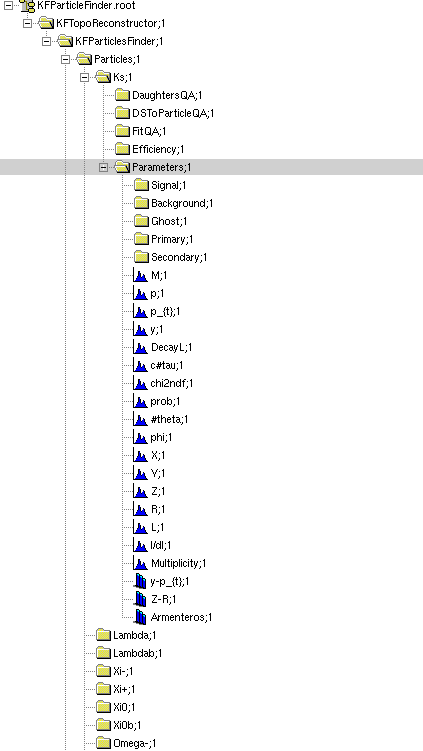
\includegraphics[width=0.42\textwidth]{particle_file.png}
	\caption{ A ROOT fájl struktúrájának egy része. }
\end{figure}
\vspace{5mm} 
\par 
\begin{figure}[H]
	\centering
	\begin{subfigure}{0.49\textwidth}
		\centering
		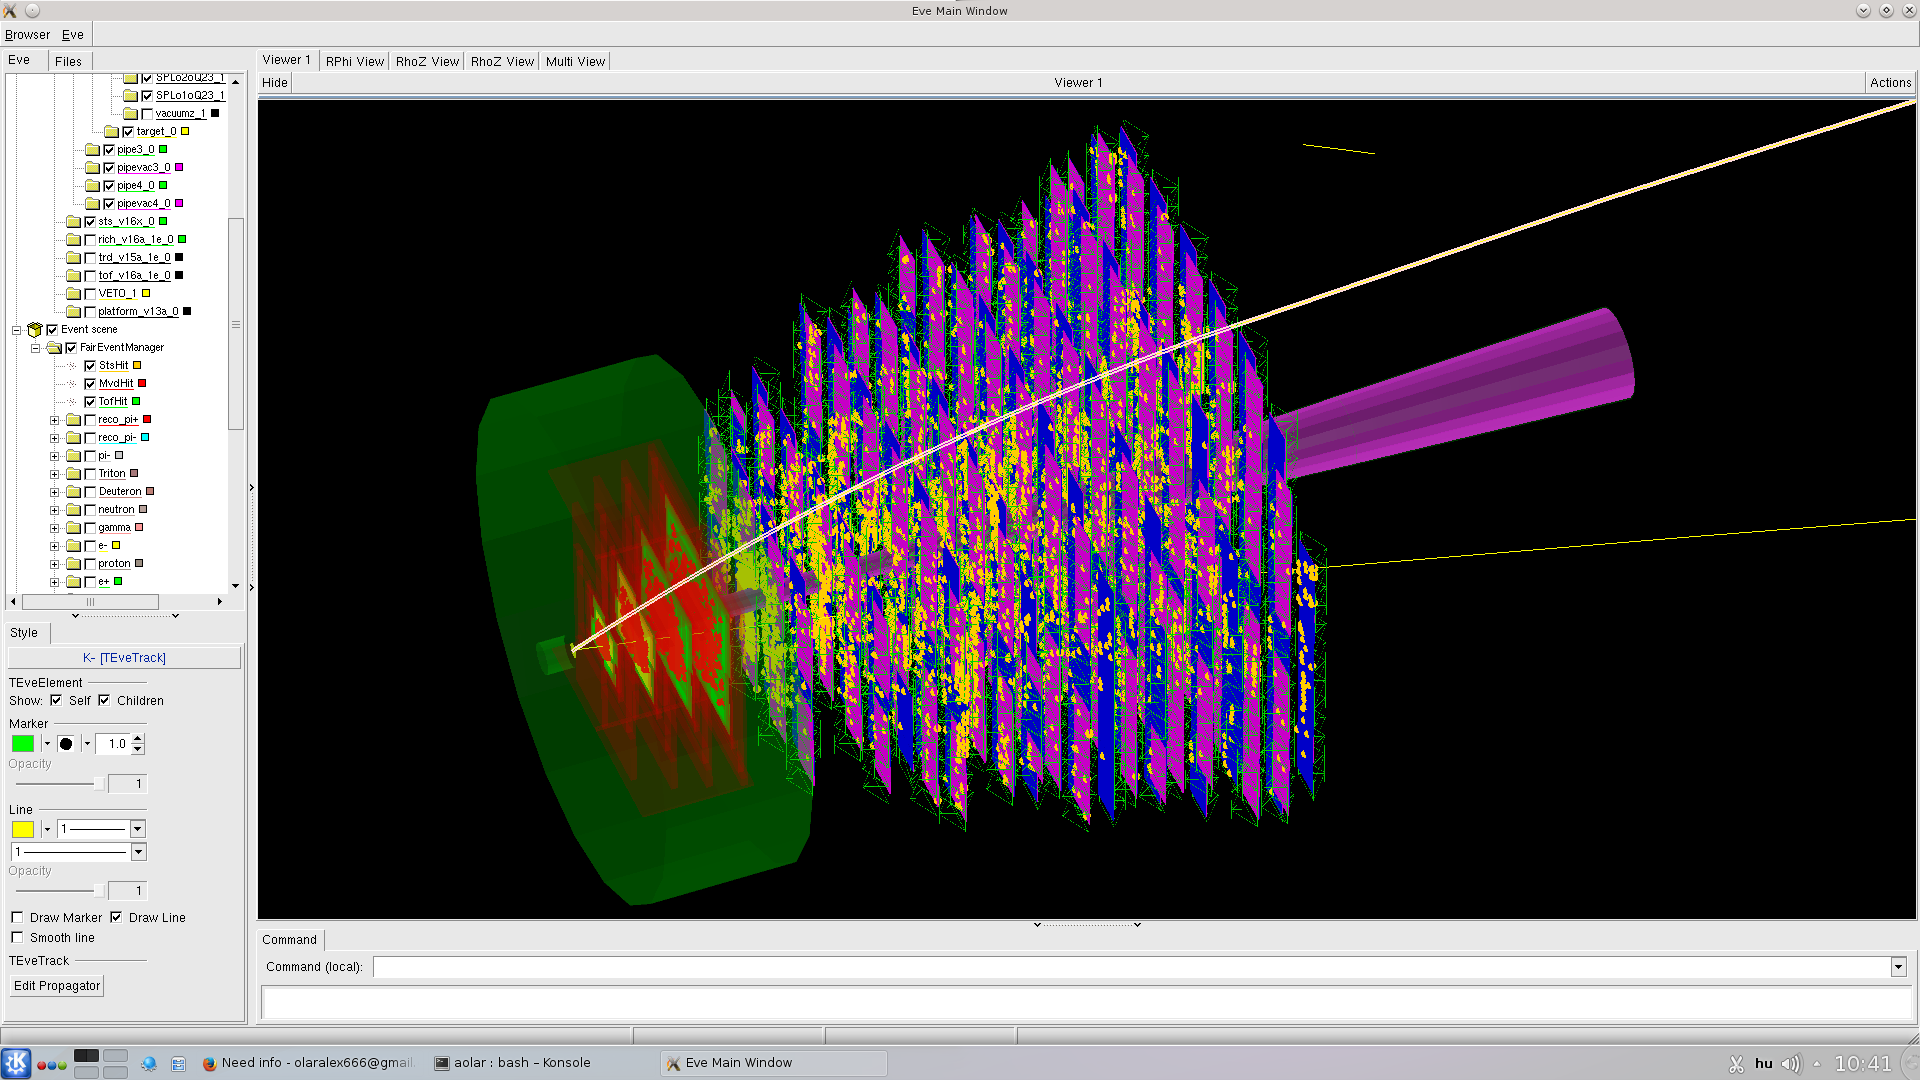
\includegraphics[width=0.95\textwidth]{reco2.png}
		\caption{ A rekonstruált pályák az MVD és STS detektorokban. }
	\end{subfigure}
	\begin{subfigure}{0.49\textwidth}
		\centering
		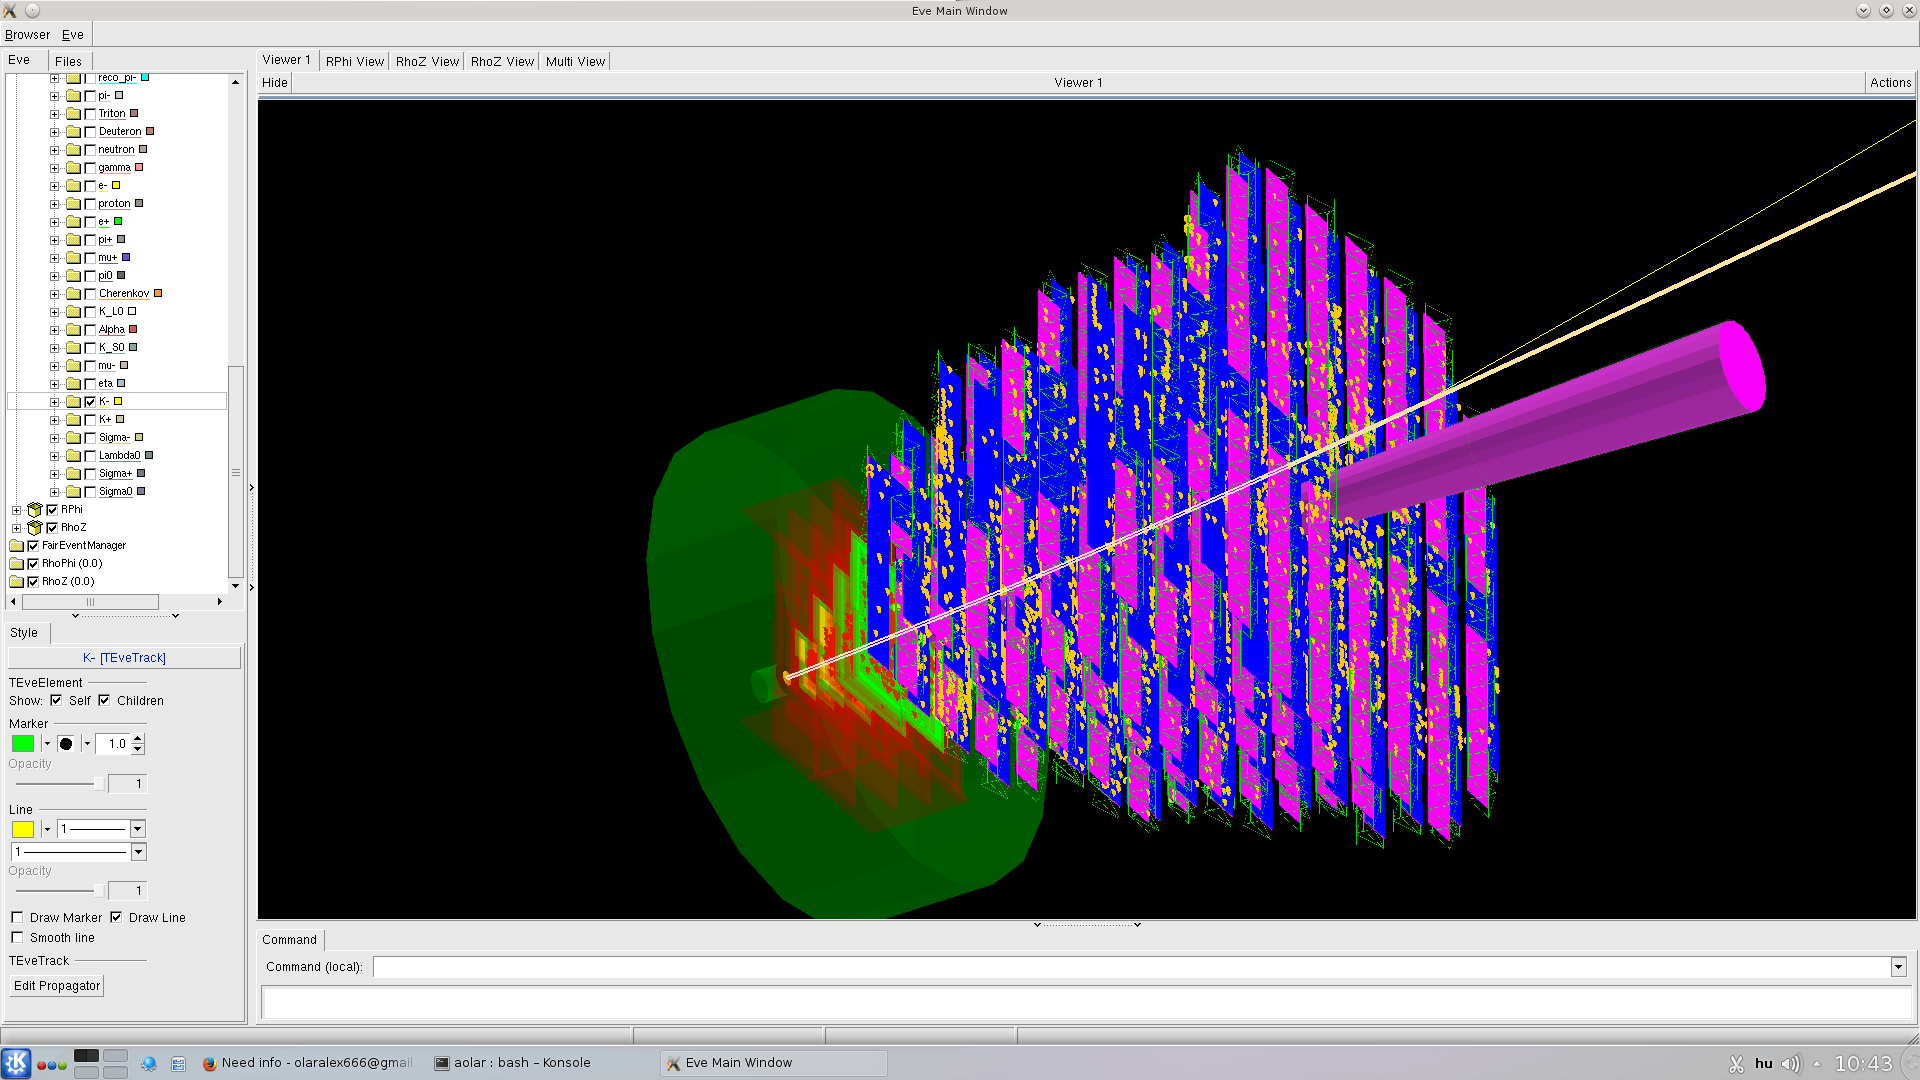
\includegraphics[width=0.95\textwidth]{reco1.png}
		\caption{ Másik szögből }
	\end{subfigure}
\end{figure}
\subsection{ How-tos}
\vspace{3mm}
\par Ahogy korábban említettem először a Monte Carlo szimulációt kell használni valmilyen bemeneti fájllal. Ez egy .root fájl vagy egy 
egyszerű ASCII fájl is lehet, a szimulációs kód képes mindkettő fogadására. Egy ilyen fájlban részecske ID-k és impulzusuk található. A kimenete 
a PHSD és a UrQMD szimulációknak általában egy .root fájl, de például a HIJING sima szöveges kimenetet produkál. A CBM szimulációnál külöböző 
függvények teszik lehetővé mindkét adattípus feldolgozását.
\vspace{3mm}
\par Megtanultam használni a jelgenerátor programot, amivel bárki, bármit küldhet a detektor szimuláció bementére. Én főként arra használtam, hogy
kontrollált körülmények között, csak $\Phi$-mezonokat küldjek be, amivel vizsgálni lehet, hogy mi lesz a program kimentén a KFParticleFinder
által kiadott .root fájlban. Ahhoz, hogy a generátor által biztosított ASCII fájlt olvasni tudja a szimuláció a következő módosítások szükségesek:
\begin{figure}[H]
	\centering
	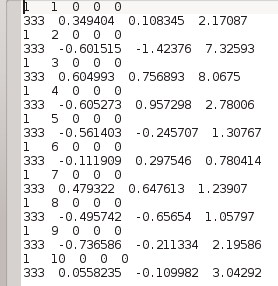
\includegraphics[width=0.5\textwidth]{input.png}
\end{figure}
\par 333 a részecske ID a $\Phi$-mezonnál. Ezután a szimuláció tudni fogja, hogy hogyan dolgozza azt fel, és képes lesz azt elbomlasztani
a megfelelő valószínűségekkel. 
\begin{lstlisting}[language=C++]
FairAsciiGenerator *SignalGen = new FairAsciiGenerator(inFile);
primGen->AddGenerator(SignalGen);
\end{lstlisting}
Fentebb a .root fájlokhoz használt $CbmUnigenGenerator$ helyett ASCII fájlok esetén ezt kell hasznáni. Még egy fontos lépes van itt. Ha szeretnénk
vizuálizálni a későbbiekben az eredményeinket, akkor engedélyeznünk kell a trajektóriák ilyen szintű mentését. Ez nyilvánvalóan nem 
hatékony hatalmas részecske számok esetén, de ha csak néhány részcskét küldünk be, akkor hasznos lehet látni, hogy hogyan is működik a 
program, esetleg hibákat is észrevehetünk.
\begin{lstlisting}[language=C++]
 // -Trajectories Visualization (TGeoManager Only )
 run->SetStoreTraj(kTRUE);  //->
 // -----------------------------------------------
\end{lstlisting}
\par Tehát a rekonstrució után, valamint a részecske felismerés végeztével, ha bekapcsoltuk a vizualizációt képesek vagyunk vizualizálni az
eseményekt. Ehhez az $eventDisplay.C$ makrót kell futtatnunk. Ez a makró az egész CBM geometriát tartalmazza, tehát az egész 
detektort átláthatjuk vele. Megjeleníthető benne az összes trajektória és a részecskék. Néhány kép arról, ahogy egy $\Phi$-mezon két kaonra bomlott:
\begin{figure}[H]
	\centering
	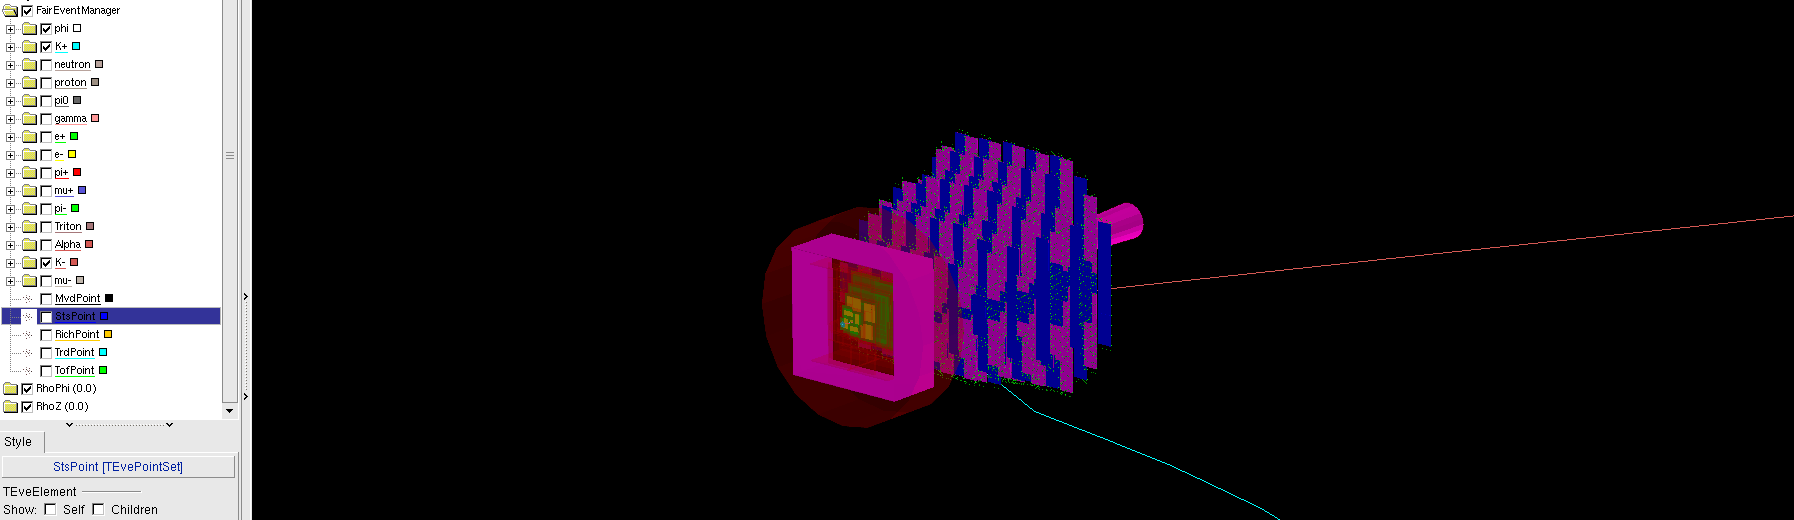
\includegraphics[width=0.85\textwidth]{k-k+decayofphi.png}
	\caption{ Vizualizáció az MVD és STS detektorokban }
\end{figure}
\subsection{ $\Phi$-mezonok generálása és a kimenő adatok elemzése}
\vspace{5mm}
\par A jelgenerátorral 2500 eseményt generáltam ahol a $\Phi$-mezonok pont a céltárgy közepében helyezkedtek el, tehát minta éppen 
ott keletkeztek volna az ütközés során. Az ilyen adatok elemzése azért fontos, mert ekkor kontorrált körülmények között, adott részecske számmal
tudjuk vizsgálni a kimenő részeskék számít, eloszlását és ebből ismeretlen kezdeti részecskénél következtethetünk a $\Phi$-mezonok számára
így a strange keltés folyamatára. 
\par A generátor makróban a bemenő nyaláb enegiáját is változtathatjuk, valamint a környezet hőmérsékletét is (mindkettő GeV-ben) és persze
azt is, hogy milyen részecskét akarunk generálni.
\begin{lstlisting}[language=C++]
double fSlope = .154; // temperature
...
double eBeam = 10.; // beam energy
double pBeam = TMath::Sqrt(eBeam*eBeam - kProtonMass*kProtonMass);
...
 const int NParticlesPerEvent = 1;
 const double kSignalMass[NParticlesPerEvent] = {1.019455};    //  mass in GeV
 const int    kSignalID[NParticlesPerEvent] =  {333};
 ...
   for (int i=0; i<NEvent; i++){
   // Generate rapidity, pt and azimuth
   outputfile<<NParticlesPerEvent<<"   "<<i + 1<<"  "<<0.<<"  "<<0.<<"  "<<0.<<endl;
   for(int j=0;j<NParticlesPerEvent;++j) {      
   double yD   = gRandom->Gaus(fYcm, fRapSigma);
   double ptD  = fThermal[j].GetRandom();
   double phiD = gRandom->Uniform(0., kTwoPi);
   
   // Calculate momentum, energy, beta and gamma
   double pxD    = ptD * TMath::Cos(phiD);
   double pyD    = ptD * TMath::Sin(phiD);
   double mtD    = TMath::Sqrt(kSignalMass[j]*kSignalMass[j] + ptD*ptD);
   double pzD    = mtD * TMath::SinH(yD);
   
   outputfile<<kSignalID[j]<<"  "<<pxD<<"  "<<pyD<<"  "<<pzD<<endl;
   
   }
   }
\end{lstlisting}
\par Jól látható, hogy ezt a makrót elég könnyű személyre szabni, tehát bárki könnyedén elkészítheti magának a számára megfelelő
bemeneti fájlt. A bemeneti fájlt az eseméynek számával és a fájl nevével át kell adni a szimulációs programnak.
\begin{lstlisting}[language=C++]
void run_mc_phi(TString inFile="Signal_phi_2500.txt", const char* setupName = "sis100_electron", Int_t nEvents = 2500)
{
  TString outFile = "sim_phi_2500.root";
  TString parFile = "param_phi_2500.root";
...
  // --- Define the target geometry -----------------------------------------
  //
  // The target is not part of the setup, since one and the same setup can
  // and will be used with different targets.
  // The target is constructed as a tube in z direction with the specified
  // diameter (in x and y) and thickness (in z). It will be placed at the
  // specified position as daughter volume of the volume present there. It is
  // in the responsibility of the user that no overlaps or extrusions are
  // created by the placement of the target.
  //
  TString  targetElement   = "Gold";
  Double_t targetThickness = 0.025;  // full thickness in cm
  Double_t targetDiameter  = 2.5;    // diameter in cm
  Double_t targetPosX      = 0.;     // target x position in global c.s. [cm]
  Double_t targetPosY      = 0.;     // target y position in global c.s. [cm]
  Double_t targetPosZ      = 0.;     // target z position in global c.s. [cm]
  Double_t targetRotY      = 0.;     // target rotation angle around the y axis [deg]
}
\end{lstlisting} 
\par A kimenet egy .root fájl, ami mint már korábban említettem adatokat tartalmaz a beütésekkel a detektor anyagban. Fontos megemlíteni, 
hogy a céltárgyat is bárminek definiálhatjuk, a helyzetét is változtathatjuk, de a mi feladatunk, hogy helyesen tegyük, mert a szimuláció lefut 
úgy is, hogy a nyaláb el sem találja a céltárgyat. 
\vspace{5mm}
\par Ezután a rekonstruciós fájlt is kissé módosítani kell, majd ez a trajektóriákat találja meg. Majd a fizika makrót kell futtatni, hogy a 
KFParticleFinder megtalálja a pályákhoz tartozó részecskéket. A kimeneti .root fájlból néhány részlet:
\begin{figure}[H]
	\centering
	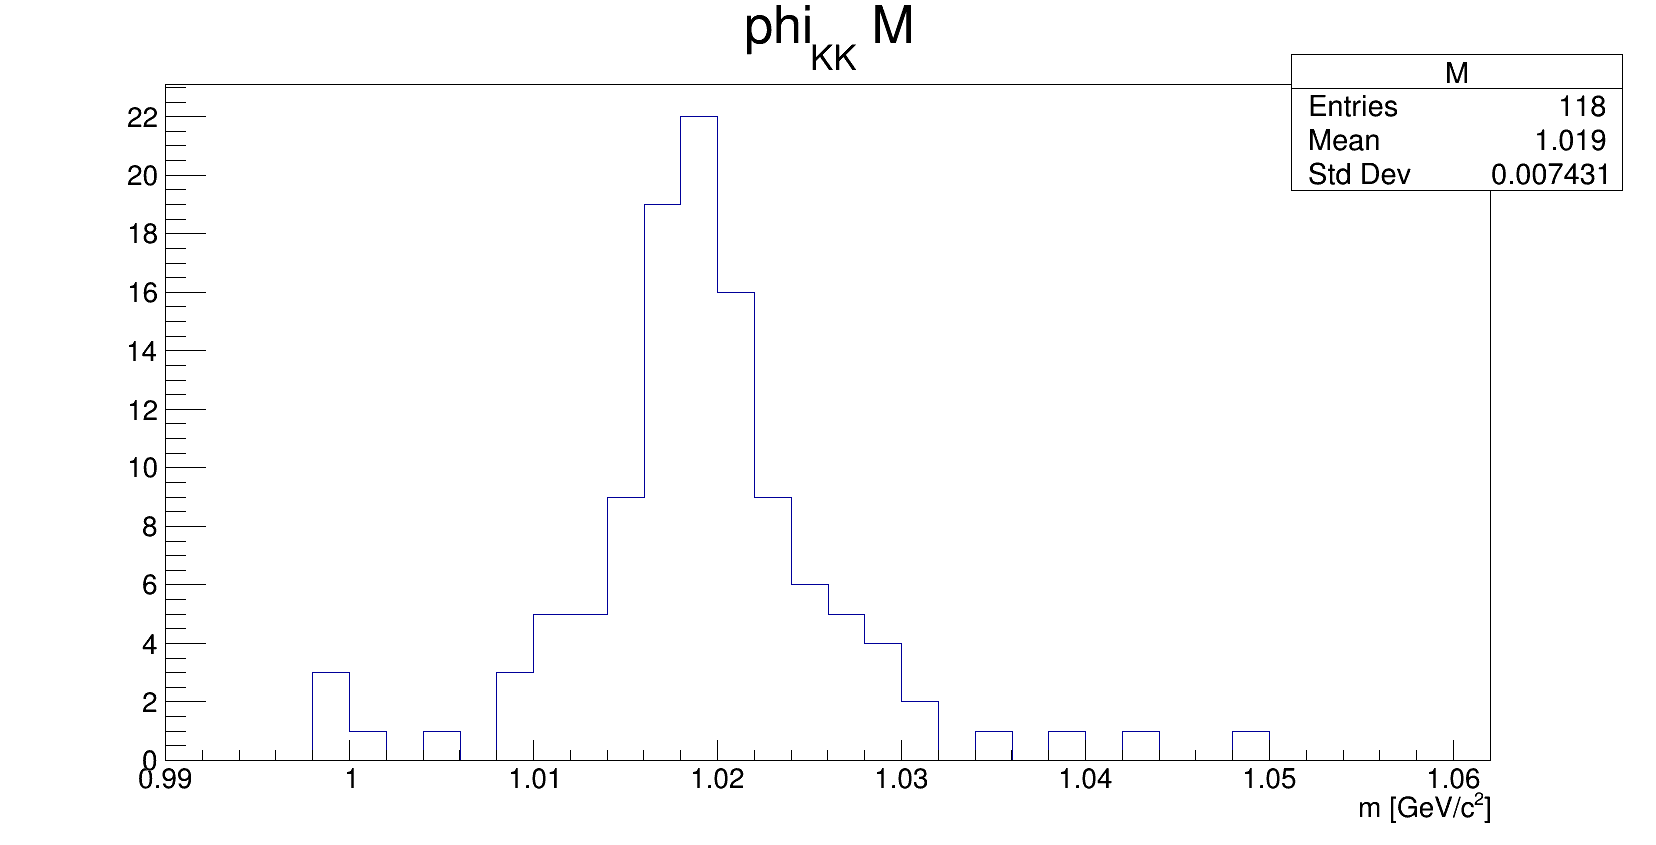
\includegraphics[width=0.5\textwidth]{phiKK_2500phi.png}
	\caption{ A kaonpárok invariáns tömegének diagramján 1.02 GeV-nél, a $\Phi$-mezon }
\end{figure}
\par A jelben 2500 esemény volt, azaz 2500 db mezont generáltam. Nagyjából 50$\%$-os eséllyel bomlottak el ezek kaon párokra, 
valamint a digitalizáció során, nagyjából 15$\%$-os hatékonysággal tudott a program rekonstruálni, azaz nagyjából 180 db rekonstruált
$\Phi$-mezonra lehet számítani a $KFParticleFinder.root$ fájlban. Mivel valószínűségekről van szó, így a fájlban lévő 120 db nem is rossz
statisztikailag.
\begin{figure}[H]
	\centering
	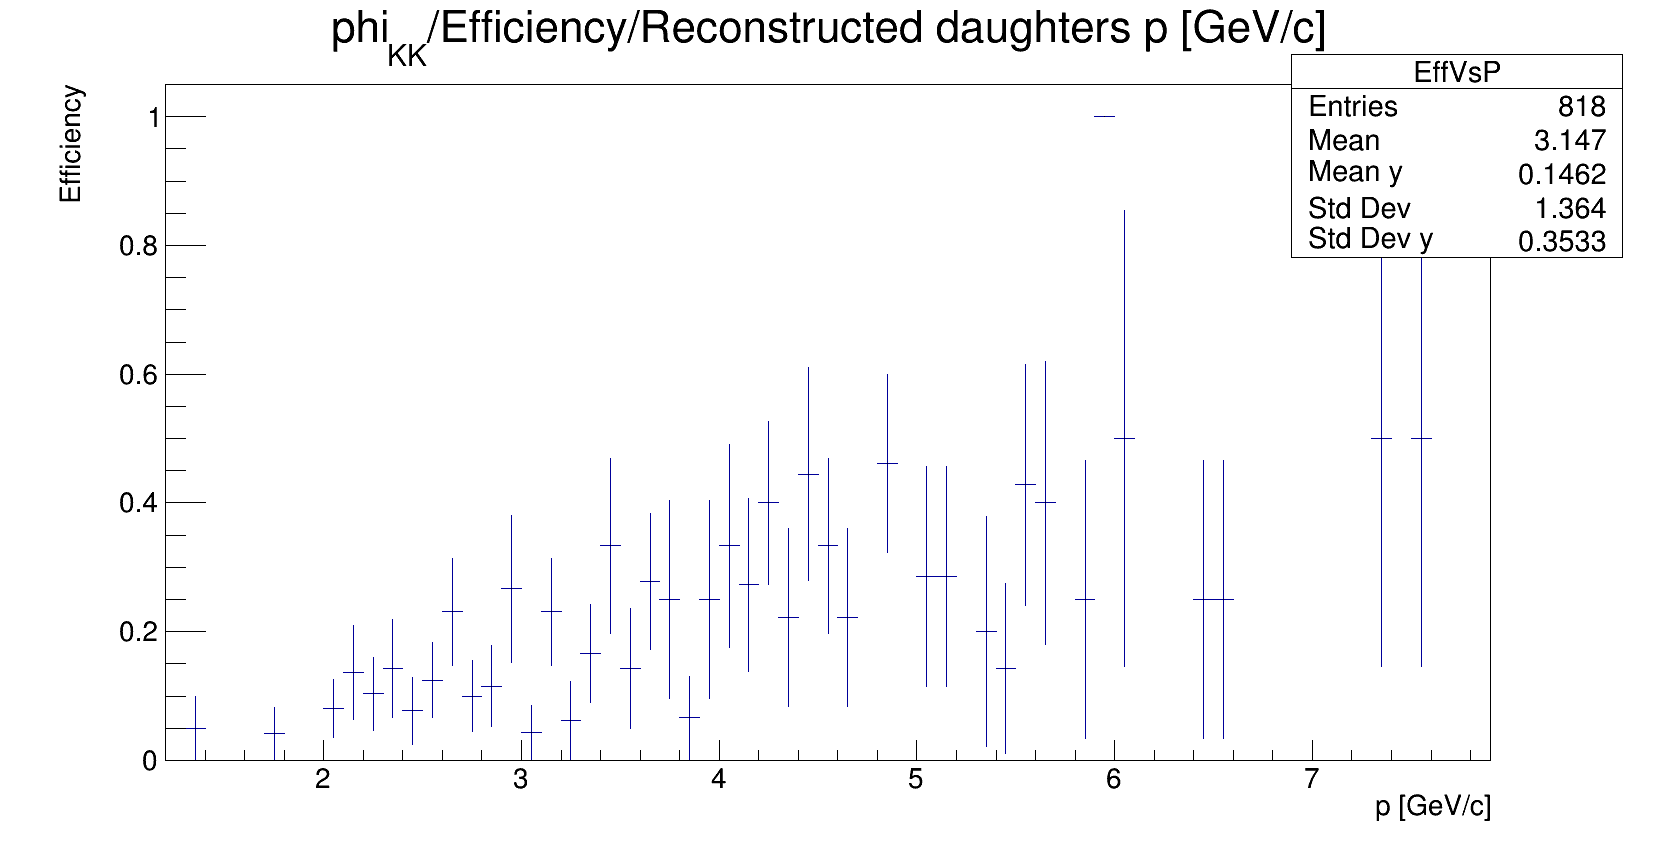
\includegraphics[width=0.5\textwidth]{reconstructed_eff_phi2500.png}
\end{figure}
\par Könnyű megtalálni azokat a részecskéket is amikké a $\Phi$-mezonok elbomlottak. Így találhatunk a bomlástermékek között
pionokat, kaonokat, $K^{0}_{S}$ részecskéket. 
\begin{figure}[H]
	\centering
	\begin{subfigure}{0.49\textwidth}
		\centering
		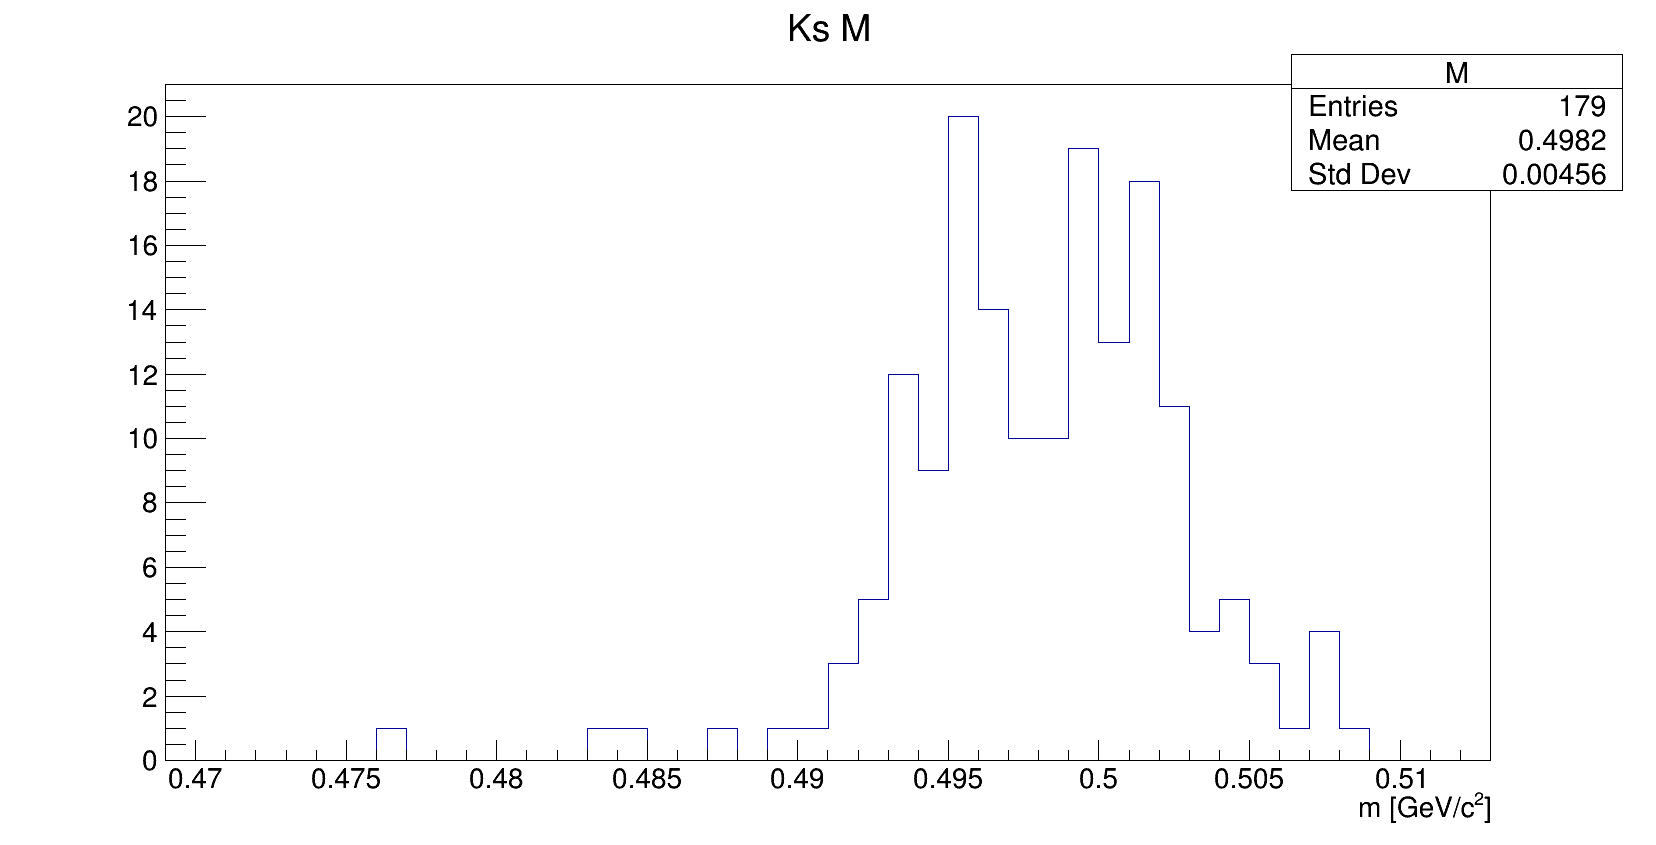
\includegraphics[width=0.95\textwidth]{kshort_phi2500.png}
		\caption{ $K^{0}_{S}$ részecskék }
	\end{subfigure}
	\begin{subfigure}{0.49\textwidth}
		\centering
		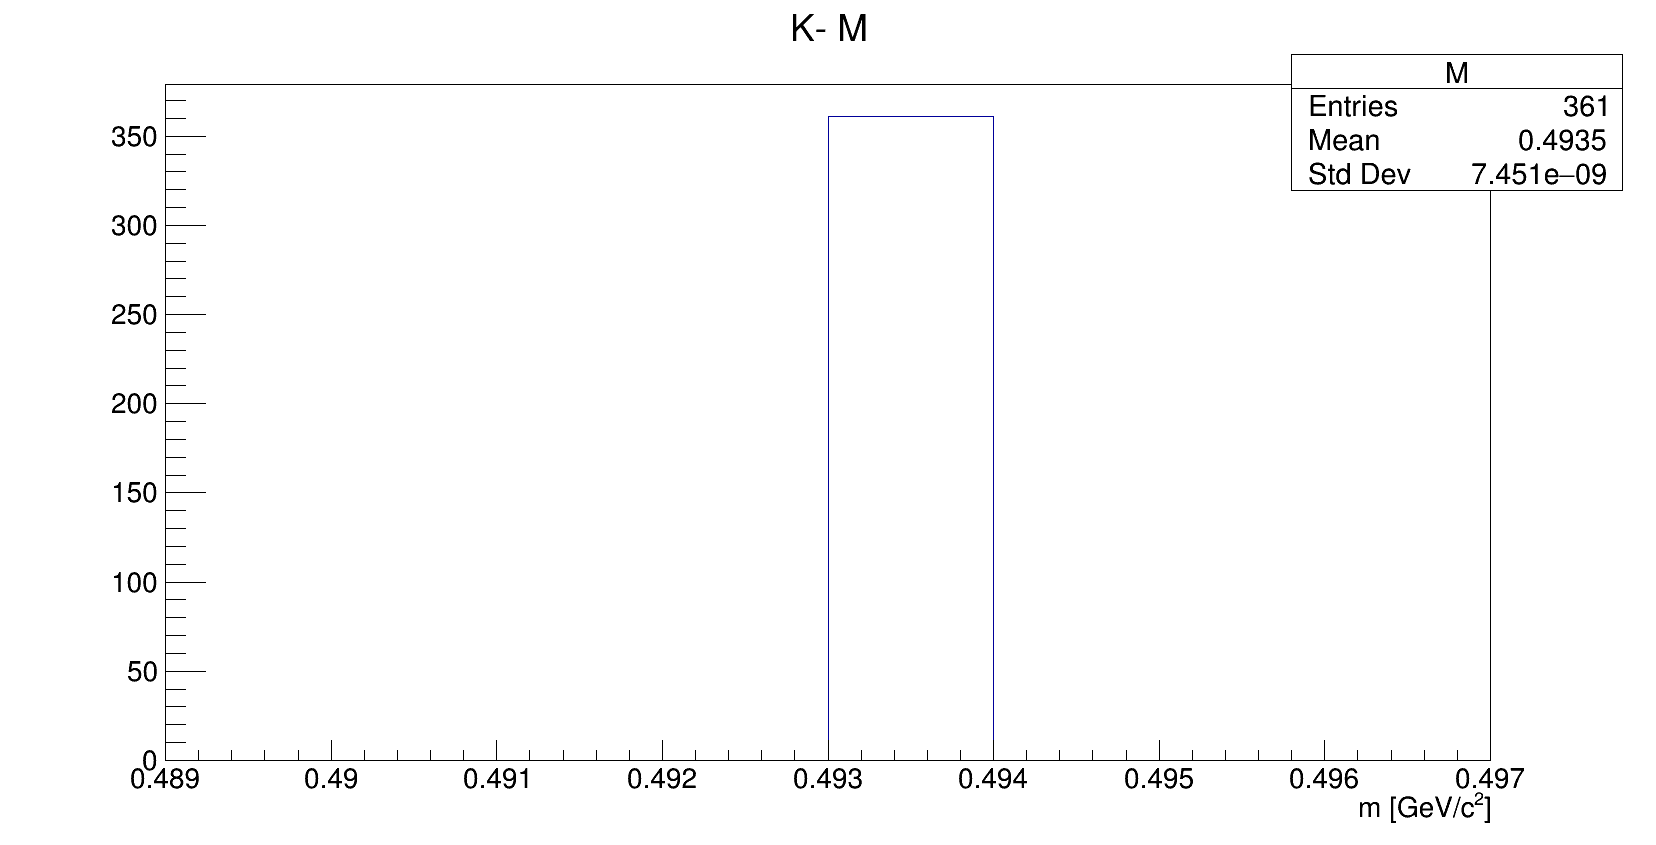
\includegraphics[width=0.95\textwidth]{k-_phi2500.png}
		\caption{ Negatív kaonok. }
	\end{subfigure}
\end{figure}
\par A pionokat itt nem tüntettem fel külön, mivel egy ilyen folyamat során azok nem adnak informatív képet, lévén, hogy nem csak a 
$\Phi$-mezon tud úgy bomlani, hogy pion is van a bomlástermékek között, de a kaonok és egyéb részecskék is, így a pionok multiplicitása igen
nagy.
\subsection{ Összegzés}
\vspace{5mm}
\par A CBM detektor képes lesz arram, hogy felismerje és megtalálja a $\Phi$-mezon bomlásokat, ezáltal a strange termelődést és a 
partonikus anyagot vizsgálni tudja. A szimulációk azt sugallják, hogy a detektor minden valószínűség szerint képes lesz detektálni a 
szükséges részecskéket a megfelelő hatásfokokkal.
\begin{thebibliography}{9}
	\bibitem{CBMbook}
	{\it The CBM Physics Book: Compressed Baryonic Matter in Laboratory Experiments} 2011 ed B Friman {\it et al} (Springer) Lect. Notes Phys.
				
	\bibitem{phiALICE} Tapia Takaki, J.~D., ALICE Collaboration 2008, Journal of Physics G Nuclear Physics, 35, 044058
				
	\bibitem{CBMexp} V.Vovchenko \and I.Vassiliev \and I.Kisel \and M.Zyzak, $\Phi$-meson production in Au+Au collisions and its feasibility in the CBM experiment, CBM Progress Report 2014
				
	\bibitem{phiRICH} Bravina, L., Csernai, L., Faessler, A., et al.\ 2003, Nuclear Physics A, 715, 665 
				
	\bibitem{phiSTAR} F. Wang, R. Bossingham, Q. Li, I. Sakrejda, and N. Xu, $\Phi$-meson reconstruction in the STAR TPC, 1998
				
	\bibitem{cbmFAIR} Hans Rudolf Schmidt Hyperons at CBM-FAIR, Journal of Physics: Conference Series
	736
\end{thebibliography}
\end{document}
